\section{Aufgabe 9: Metropolis-Hastings-Algorithmus}
\subsection{a)}
Da eine gaußförmige Verteilung eine symmetrische Verteilung ist, gilt:
\begin{equation*}
  g(x_j|x_i) = g(x_i|x_j)
\end{equation*}
daher folgt für die Übergangswahrscheinlichkeit des Metropolis-Hastings-Algorithmus:
\begin{equation*}
  M_{\symup{i->j}} = \symup{min}\left(1, \frac{f(x_j)}{f(x_i)} \frac{g(x_j|x_i)}{g(x_i|x_j)}\right) =
  \symup{min}\left(1, \frac{f(x_j)}{f(x_i)}\right)
\end{equation*}
dieser Ausdruck entspricht widerum dem Metropolis-Algorithmus.

\subsection{b) und c)}
Siehe Quellcode.
Das normierte Histogramm mit der zugrundeliegenden Wahrscheinlichkeitsverteilung ist in Abbildung \ref{abb:1} zu sehen.
\begin{figure}[h]
  \centering
  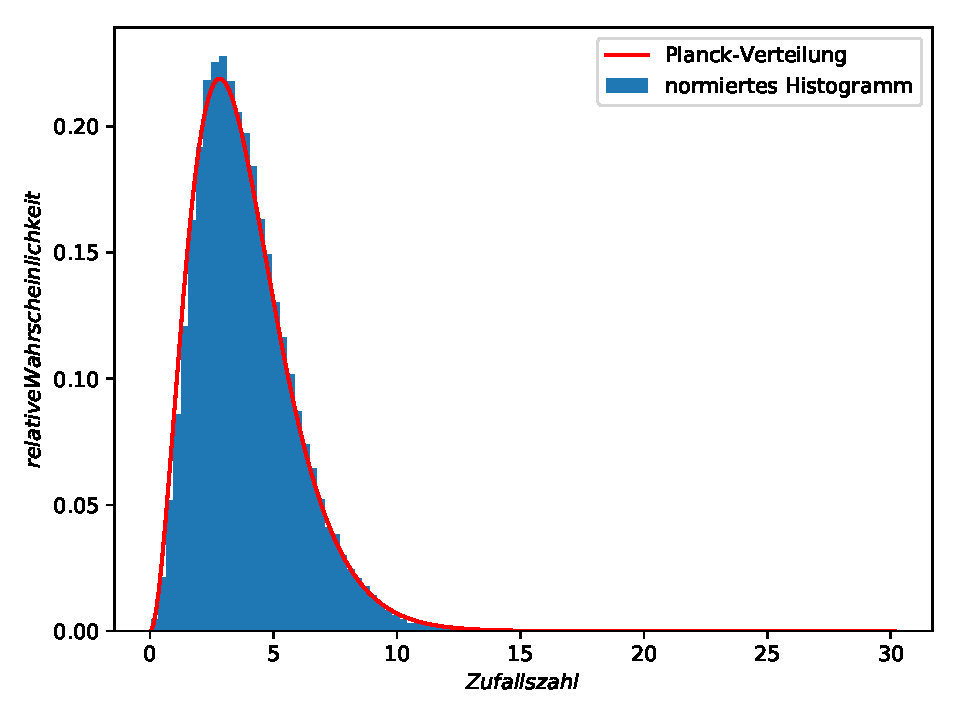
\includegraphics{Metropolis.pdf}
  \caption{Normiertes Histogramm mit Wahrscheinlichkeitsverteilung.}
  \label{abb:1}
\end{figure}

\subsection{d)}
Der "Trace Plot" ist in Abbildung \ref{abb:2} zu sehen. In Abbildung \ref{abb:3} ist noch einmal ein Traceplot zu sehen,
der nur die ersten 200 Schritte anzeigt.
In  \ref{abb:3} lässt sich die "Burn-In"-Phase des Algorithmus gut erkennen, da der Startwert
nicht in der Nähe des Maximums der Verteilung liegt.
\begin{figure}[h]
  \centering
  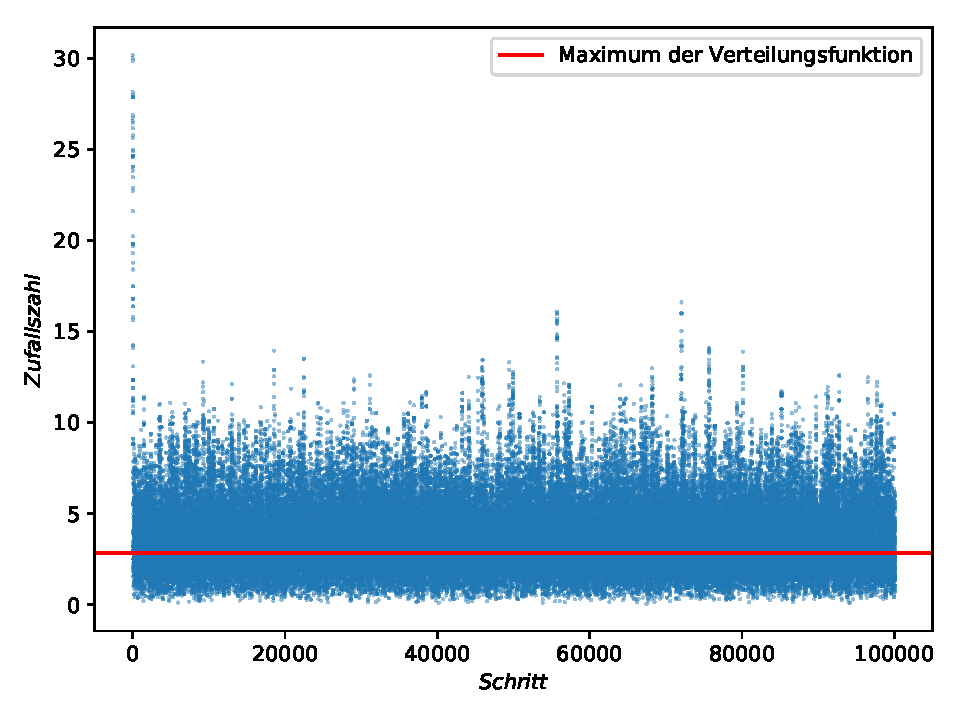
\includegraphics{MetropolisSchritte.pdf}
  \caption{Trace Plot.}
  \label{abb:2}
\end{figure}
\begin{figure}[h]
  \centering
  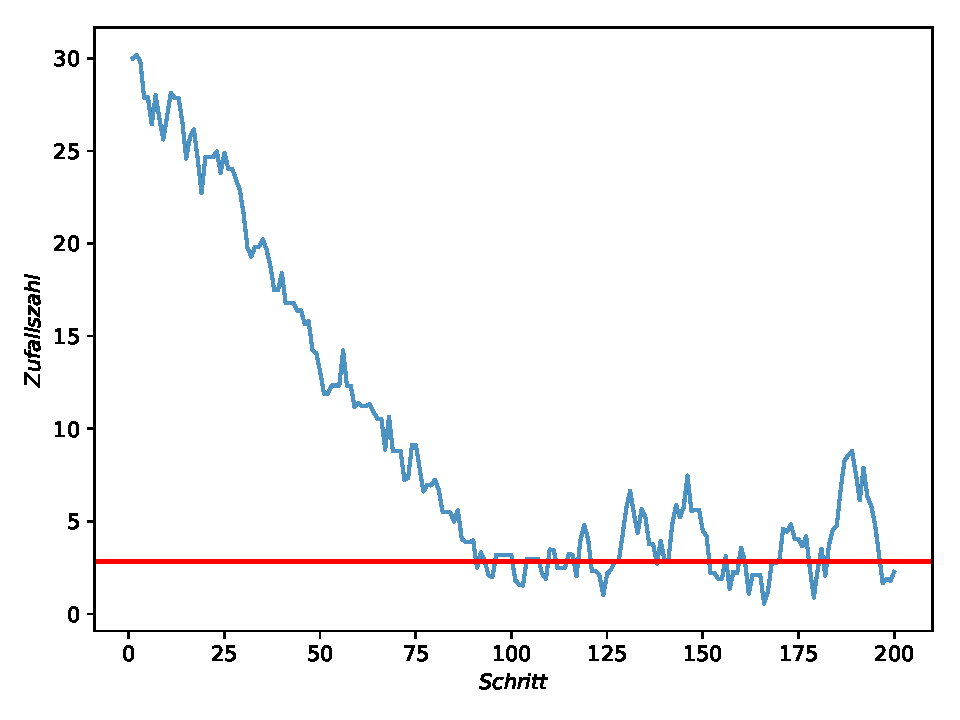
\includegraphics{MetropolisSchritte2.pdf}
  \caption{Trace Plot Ausschnitt.}
  \label{abb:3}
\end{figure}
